\chapter{Geometria delle aree}
%\addcontentsline{toc}{chapter}{B. Geometria delle aree} % Aggiunge il capitolo all'indice
%\renewcommand{\theequation}{B\arabic{equation}}
\setcounter{chapter}{0} % Reset del contatore delle equazioni
\renewcommand{\thesection}{B.\arabic{section}}
\setcounter{section}{0} % Reset del contatore delle sezioni


\section{Momento statico, baricentro, momento d'inerzia}
Sia $\Omega$ un dominio di $\Ec^2$; fissiamo un sistema di riferimento ortonormale $\{O; \eb_1, \eb_2\}$ e sia $\pb= x_1 \eb_1+x_2 \eb_2$ la posizione del generico punto di $\Omega$.

\begin{figure}[h!]
	\centering
	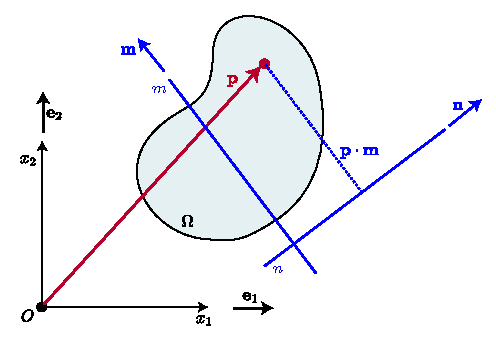
\includegraphics[scale=1.3]{figure/geometria_aree/area}
	\caption{}
	\label{fig:area}
\end{figure}

Consideriamo due assi ortogonali $n$ e $m$ e i versori che ne individuano le direzioni $\nb$ e $\mb $.
Il  \textit{momento statico} (o del primo ordine)  di $\Omega$ rispetto all'asse $n$ è una misura che descrive quanto ``distribuita'' è l'area rispetto a quell'asse. Immaginiamo di dividere $\Omega$ in piccole porzioni (come dei rettangolini);  per ogni porzione, consideriamo il prodotto dell'area della porzione per la sua distanza verticale dall'asse n; il momento statico rispetto all'asse $n$ è la somma di tutti questi prodotti.

In maniera più precisa, essendo la distanza da $n$ del generico punto $\pb$ data da $\pb \cdot \mb$, definiamo il momento statico rispetto a $n$ come
\begin{definition}
	\begin{equation}
S_n\coloneqq  \sb \cdot \mb, \qquad \sb \coloneqq \int_{\Omega}\pb,
\end{equation}
\end{definition}
dove $\sb$ è il vettore \textit{momento statico}.
La distanza da $n$ così definita ha un segno, che è positivo se $\pb$ si trova dalla stessa parte della direzione individuata da $\mb $.

In particolare, i momento statici rispetto agli assi $x_1$ e $x_2$ sono
\begin{equation}
	S_1 =\sb \cdot \eb_2= \int_{\Omega}x_2, \qquad S_2 =\sb \cdot \eb_2= \int_{\Omega}x_1.
\end{equation}


Si definisce \textit{baricentro} o \textit{centro d'area} $G$ il punto individuato dal vettore
\begin{equation}
	\pb(G)\coloneqq \frac{\sb}{A},
\end{equation}
dove $A$ è l'area di $\Omega$.
Dunque le coordinate del  baricentro sono individuabili come
\begin{equation}
	x_{1}(G)=\frac{S_2}{A}, \qquad x_{2}(G)=\frac{S_1}{A}.
\end{equation}


Il  \textit{momento d'inerzia} (o del secondo ordine)  di $\Omega$ rispetto all'asse $n$ è definito come
\begin{definition}
	\begin{equation}
J_n =\int_{\Omega}(\pb \cdot\mb)^2.
\end{equation}
\end{definition}
Dunque, anziché pesare la distanza da $n$, ne pesiamo adesso il quadrato. 
La quantità
\begin{definition}
	\begin{equation}
J_{nm}=\int_{\Omega}(\pb \cdot\nb)(\pb \cdot\mb)
\end{equation}
\end{definition}
definisce il \textit{momento centrifugo} (o misto) e 
\begin{definition}
	\begin{equation}
		J_o=\int_{\Omega}|\pb|^2
	\end{equation}
	\end{definition}
il \textit{momento polare}.
In particolare, abbiamo
\begin{equation}
J_1=\int_{\Omega}x_2^2, \qquad J_2=\int_{\Omega}x_1^2, \qquad J_{12}=\int_{\Omega}x_1 x_2, \qquad J_o=\int_{\Omega}x_1^2+x_2^2=J_1+J_2.
\end{equation}

Poiché
\begin{equation}
(\pb \cdot\mb)^2=\pb \otimes \pb \cdot \mb\otimes \mb = \pb \otimes \pb\cdot (\Ib - \nb \otimes \nb),
\end{equation}
visto che possiamo scrivere l'identità come $\Ib =\nb\otimes \nb +\mb \otimes \mb$, possiamo scrivere
\begin{equation}
	J_n =\int_{\Omega}|\pb|^2-\pb \otimes \pb\cdot \nb \otimes \nb=\Jb \cdot \nb \otimes \nb=\Jb \nb \cdot \nb,
\end{equation}
dove abbiamo definito il \textit{tensore d'inerzia}
\begin{definition}
\begin{equation}
\Jb \coloneqq \int_{\Omega}|\pb|^2 \Ib -\pb \otimes \pb.
\end{equation}
\end{definition}

Il tensore d'inerzia è chiaramente simmetrico e definito positivo. Valutiamone le componenti:
\begin{equation}
\eb_1\cdot \Jb \eb_1=\int_{\Omega}|\pb|^2-(\pb\cdot \eb_2)^2=\int_{\Omega}x_2^2=:J_1
\end{equation}
è il momento d'inerzia rispetto all'asse $1$. Analogamente otteniamo $\eb_2\cdot \Jb \eb_2=J_2$ e 
\begin{equation}
	\eb_1\cdot \Jb \eb_2=\int_{\Omega}-\pb \cdot \eb_1 \pb \cdot \eb_2=-\int_{\Omega}x_1 x_2=-J_{12},
\end{equation}
mentre
\begin{equation}
\Jb \eb_3\cdot\eb_{3}=\int_{\Omega}|\pb|^2=J_o\eb_3,
\end{equation}
dove $J_o$ è il momento d'inerzia polare della regione $\Omega$, l’autovalore corrispondente all’autovettore $\eb_3$.
Dunque la matrice rappresentativa del tensore d'inerzia è
\begin{equation}
	[\Jb]=\begin{bmatrix}J_{1}&-J_{12}&0\\-J_{12}&J_{2}&0\\0 & 0 & J_o\end{bmatrix}.
\end{equation}
Poiché $\Jb$ è simmetrico e definito positivo i suoi autovalori sono tutti positivi. Si può dunque dare di $\Jb$ la rappresentazione spettrale
\begin{equation}
	\Jb = \sum_{\alpha=1}^{2}\gamma_\alpha\gb_\alpha\otimes \gb_\alpha+J_o\eb_{3}\otimes\eb_{3}, \qquad J_o=\gamma_1+\gamma_2>0.
\end{equation}
Possiamo quindi fissare l'attenzione sul tensore d'inerzia ridotto
\begin{equation}
\Jb_r\coloneqq \Jb -J_o\,\eb_{3}\otimes\eb_{3}.
\end{equation}
Di qui in avanti, salvo avviso contrario, scriveremo $\Jb$ intendendo $\Jb_r$.

Sia le componenti del vettore momento statico $\sb$ sia quelle del tensore d’inerzia $\Jb$ dipendono ovviamente dal sistema di riferimento scelto. Vediamo nel seguito come cambiano se si sceglie un differente sistema di riferimento.

\section{Trasformazioni di coordinate per traslazione}
Consideriamo un nuovo sistema di riferimento $\{O', \eb_1, \eb_2\}$ ottenuto dal primo tramite una traslazione dell'origine: $O'=O+\db$, con $\db =d_1 \eb_1+ d_2 \eb_2$.

\begin{figure}[h!]
	\centering
	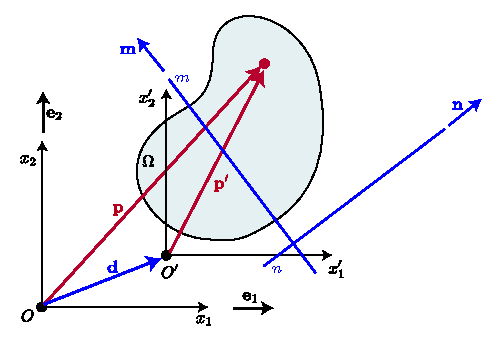
\includegraphics[scale=1.3]{figure/geometria_aree/traslazione}
	\caption{}
	\label{fig:traslazione}
\end{figure}

Allora si ha evidentemente
\begin{equation}
	\pb =\pb'+\db
\end{equation}
 e dunque,  
 integrando su $\Omega,$ si ottiene che il momento statico vale
 \begin{equation}
 \sb'=\sb -A \db.
 \end{equation}
In particolare, otteniamo
\begin{equation}
S'_n=S_n-A\db\cdot \nb
\end{equation}
e
\begin{equation}
S'_1=S_1-A d_1, \qquad S'_2=S_2-A d_2.
\end{equation}
Se il vettore $\db$ porta la nuova origine $O'$ nel baricentro $G$ di $\Omega$, ovvero se $\db \equiv \pb (G) $, si ottiene che
\begin{equation}
\sb'=\mathbf{0},
\end{equation}
e dunque i momenti statici rispetto ad assi baricentrici sono sempre nulli.

Per quanto riguarda i momenti d'inerzia, si ha
\begin{equation}
\begin{aligned}
&	J_n=\int_{\Omega}(\pb'\cdot \mb)^2+(\db \cdot \mb)^2+2 (\pb' \cdot \mb)(\db\cdot \mb)=J'_n+A (\db \cdot \mb)^2+2S'_n(\db\cdot \mb),\\
&	J_{nm}=\int_{\Omega}\big((\pb'+\db) \cdot\nb\big)\big((\pb'+\db) \cdot\mb\big)=J'_{nm}+S_m'(\db \cdot \mb)+S_n'(\db \cdot \nb)+A(\db \cdot \nb)(\db \cdot \mb).
\end{aligned}
\end{equation}
In particolare, se  il vettore $\db$ porta la nuova origine $O'$ nel baricentro $G$, 
\begin{equation}
	J_n=J'_n+A (\db \cdot \mb)^2, \qquad J_{nm}=J'_{nm}+A(\db \cdot \nb)(\db \cdot \mb),
\end{equation}
e
\begin{definition}
	\begin{equation}\label{Steiner}
	J_1(G)=J_1+Ax_2^2(G), \qquad 	J_2(G)=J_2+Ax_1^2(G), \qquad J_{12}=J_{12}(G)+A x_1(G)x_2(G),
\end{equation}
\end{definition}
dove con $J_1(G)$, $J_2(G)$ e $J_{12}(G)$ si sono indicati i momenti d'inerzia e il momento centrifugo di $\Omega$ rispetto ad assi paralleli a $\{x_1, x_2\}$ e centrati in $\pb (G)$, per questa ragione detti \textit{centrali}. Il risultato \eqref{Steiner} va sotto il nome di \textit{Teorema di Huyghens}.


\section{Trasformazioni di coordinate per rotazione}
Consideriamo adesso un sistema di riferimento $\{O; \eb_1', \eb_2'\}$ ottenuto dal primo tramite rotazione degli assi di un angolo $\vartheta$
\begin{equation}
\eb_1'=\cos\vartheta\eb_1+\sin\vartheta\eb_2, \qquad \eb_2'=-\sin\vartheta\eb_1+\cos\vartheta\eb_2.
\end{equation}
La relazione tra le coordinate dei due sistemi è
\begin{equation}
x_1'=\pb\cdot \eb_1'=x_1\cos\vartheta+x_2\sin\vartheta, \qquad x_2'=\pb\cdot \eb_2'=-x_1\sin\vartheta+x_2\cos\vartheta.
\end{equation}
Da questa si trova facilmente
\begin{equation}
	\begin{aligned}S'_{1}=-S_{x_2}\sin\vartheta+S_{x_1}\cos\vartheta,\quad&S'_{2}=S_{x_2}\cos\vartheta+S_{x_1}\sin\vartheta,\end{aligned}
\end{equation}
e
\begin{equation}
	S_{1}=S'_{1}\left.\cos\vartheta+S'_{2}\sin\vartheta,\quad\right.\quad S_{2}=-S'_{1}\sin\vartheta+S'_{_2}\cos\vartheta.
\end{equation}
Analogamente, per i momenti d'inerzia si ottiene
\begin{equation}\label{Jruot}
	\begin{aligned}
		J'_{1}& =J_1\cos^2\vartheta+J_2\sin^2\vartheta-2J_{12}\sin\vartheta\cos\vartheta, \\
		J'_{2}& =J_1\sin^2\vartheta+J_2\cos^2\vartheta+2J_{12}\sin\vartheta\cos\vartheta, \\
		J'_{12}& =J_1\sin\vartheta\cos\vartheta-J_2\sin\vartheta\cos\vartheta+J_{12}(\cos^2\vartheta-\sin^2\vartheta). 
	\end{aligned}
\end{equation}
Si dicono \textit{assi principali d’inerzia} gli assi cartesiani rispetto ai quali il momento centrifugo è nullo. Se uno dei due assi cartesiani è un asse di simmetria della regione, allora gli assi sono principali d’inerzia. In assenza di simmetrie possiamo trovare gli assi principali d’inerzia tramite un’opportuna rotazione. Infatti le \eqref{Jruot} possono essere riscritte come
\begin{definition}
	\begin{equation}\label{Jp}
	\begin{aligned}
		J'_{1}& =J_{1}\cos^{2}\vartheta+J_{2}\sin^{2}\vartheta-J_{12}\sin(2\vartheta), \\
		J'_{2}& =J_1\sin^2\vartheta+J_2\cos^2\vartheta+J_{12}\sin(2\vartheta), \\
		J'_{12}& =\frac{J_1-J_2}2\sin(2\vartheta)+J_{12}\cos(2\vartheta),
	\end{aligned}
\end{equation}
\end{definition}
noto come\textit{ Teorema di Steiner}, da cui ci accorgiamo che $	J'_{12}=0$ se e solo se 
\begin{equation}
\frac{J_{1}-J_{2}}{2}\sin(2\vartheta)+J_{12}\cos(2\vartheta)=0.
\end{equation}
Se $J_1=J_2$ allora necessariamente $\cos(2\vartheta)=0$ e quindi $\vartheta=\pm \pi/4$, mentre se $J_1\neq J_2$ si ha
\begin{equation}\label{thprinc}
	\tan(2\vartheta)=\frac{2J_{12}}{J_{2}-J_{1}}\quad\mathrm{~e~}\quad\vartheta=\frac{1}{2}\arctan\frac{2J_{12}}{J_{2}-J_{1}}.
\end{equation}
Questo è l’angolo di cui si deve ruotare gli assi $\{x_1,x_2\}$ per ottenere gli assi principali d’inerzia.  I momenti d’inerzia $J_\xi$, $J_\eta$ rispetto agli assi principali d’inerzia vengono detti\textit{ momenti principali d’inerzia}. Tali momenti possono essere calcolati sostituendo il valore di $\vartheta$ di \eqref{thprinc} in \eqref{Jp}; con un po' di fatica, si ottiene
\begin{equation}\label{Jxieta}
	J_\xi=\frac{J_1+J_2}2+\sqrt{\left(\frac{J_2-J_1}2\right)^2+J_{12}^2}, 	J_\eta=\frac{J_1+J_2}2+\sqrt{\left(\frac{J_2-J_1}2\right)^2+J_{12}^2}.
\end{equation}

D'altra parte, i momenti principali d'inerzia, corrispondo agli autovalori del tensore d'inerzia e le direzioni principali sono individuate dai corrispondenti autovettori.
Infatti, per determinare le autocoppie di $\Jb$, occorre determinare le radici del polinomio caratteristico
\begin{equation}
\det\,	\begin{pmatrix}J_1-\lambda&-J_{12}\\\cdot&J_\mathrm{2}-\lambda\end{pmatrix}=\lambda^2-(J_{1}+J_{2})\lambda+(J_{1}J_2-J_{12}^2),
\end{equation}
che coincidono con \eqref{Jxieta}.

Per trovare l'autovettore $\xib$ associato a $J_\xi$ basta risolvere il sistema
\begin{equation}
\begin{cases}
(J_1-J_\xi)\xi_1-J_{12}\xi_2=0\\
\xi_1^2+\xi_2^2=1,
\end{cases}
\end{equation}
ottenendo
\begin{equation}
\xi_1=\sqrt{\frac{J_{12}^2}{(J_1-J_\xi)^2+J_{12}^2}}, \qquad \xi_2=\sqrt{\frac{(J_1-J_\xi)^2}{(J_1-J_\xi)^2+J_{12}^2}}, 
\end{equation}
Analogamente si procede per trovare l'autovettore $\boldsymbol{\eta}$ corrispondete all'autovalore $J_\eta$, ottenendo
\begin{equation}
 \eta_1=\sqrt{\frac{(J_2-J_\eta)^2}{(J_2-J_\eta)^2+J_{12}^2}},  \qquad
	\eta_2=\sqrt{\frac{J_{12}^2}{(J_2-J_\eta)^2+J_{12}^2}}. 
\end{equation}

Le formule appena dedotte hanno una  versione grafica, dovuta a Otto Mohr. Il cerchio di Mohr relativo ad  un tensore d'inerzia ha 
\begin{equation}
{\rm centro}\equiv \left( \frac{J_1+J_2}{2},0 \right) \quad {\rm} \quad {\rm raggio}\equiv\sqrt{\left(\frac{J_1-J_2}{2}\right)^2+J_{12}^2}.
\end{equation}

\begin{figure}[h]
	\centering
	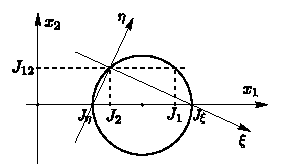
\includegraphics[scale=1.4]{figure/geometria_aree/mohr}
	\caption{Cerchio di Mohr per il tensore d'inerzia.}
	\label{fig:mohr}
\end{figure}

Si vede facile vedere che, una volta costruito questo cerchio, i momenti principali si ottengono come come intercette con l’asse orizzontale e che gli assi principali hanno le direzioni delle rette mutuamente ortogonali che congiungono tali intercette con il punto sul cerchio di coordinate $(J_{2}, J_{12})$.

Ad esempio, si vede dalla figura che la retta che passa per i punti $(J_2, J_{12} )$ e $(J_\eta,0)$ ha coefficiente angolare $J_{12}/(J_2-J_\eta)$, pari alla pendenza dell'autovettore $\boldsymbol{\eta}$; questa retta fornisce quindi la posizione dell’asse principale centrale $\eta$ rispetto all’asse $x_1$.

\section{Le simmetrie}
Riportiamo alcune utili proprietà che si presentano in regioni con simmetrie.
\begin{enumerate}
	\item Il baricentro appartiene agli assi di simmetria.
	\item Gli assi di simmetria sono assi principali.
	\item Se sono presenti tre o più assi di simmetria, tutti gli assi sono principali. Ad esempio nel cerchio o nel quadrato.
	\item Se $J_1=J_2$ e contemporaneamente $J_{12}=0$, tutti gli assi sono principali.
	\item Se $J_1\neq J_2$ e contemporaneamente $J_{12}=0$, gli assi 1 e 2 sono principali.
	\item Se $J_1=J_2$ e $J_{12}\neq0$ gli assi principali sono a $\pi/4$.
\end{enumerate}

\section{Le sezioni sottili}
\lipsum[1]

\section{L'ellisse d'inerzia}
Definiamo \textit{raggi d'inerzia} (o giratori d'inerzia) relativi agli assi 1 e 2  le quantità
\begin{equation}
\rho_1\coloneqq \sqrt{\frac{J_1}{A}}, \qquad \rho_2\coloneqq \sqrt{\frac{J_2}{A}};
\end{equation}
indichiamo inoltre con
\begin{equation}
\rho_\xi =\sqrt{\frac{J_\xi}{A}}, \qquad \rho_\eta =\sqrt{\frac{J_\eta}{A}},
\end{equation}
i \textit{raggi d'inerzia principali}. Nel sistema di riferimento principale centrale l'equazione
\begin{equation}
	\frac{\xi^2}{\rho_\eta^2}+\frac{\eta^2}{\rho_\xi^2}=1
\end{equation}
definisce l'\textit{ellisse principale d'inerzia}. 


%Scegliendo $\xib \equiv \eb_1$ e $\boldsymbol{\eta} \equiv \eb_2$, il generico punto $\xb$ dell'ellisse è dunque
%\begin{equation}
%\xb=\rho_\eta\,\cos\alpha\,\eb_1+\rho_\xi\,\sin \alpha\,\eb_2, \qquad 0\leq \alpha<2\pi.
%\end{equation}
%Il vettore unitario tangente all'ellisse in $\xb$ è
%
%\begin{equation}
%\mb =\frac{\xb '}{|\xb|}=-\frac{\rho_\eta}{\sqrt{\rho_\xi^2+\rho_\eta^2}}\sin\alpha \,\eb_1+\frac{\rho_\xi }{\sqrt{\rho_\xi^2+\rho_\eta^2}}\cos\alpha\,\eb_2.
%\end{equation}

Una qualunque conica non degenere, e dunque anche l'ellisse, determina una corrispondenza biunivoca tra una coppia punti e rette e tra una coppia di rette  definita \textit{polarità}. Punti e rette o rette e rette che si corrispondono nella polarità vengono dette \textit{coniugate}.

Vediamo nel seguito alcune caratteristiche utili di questa corrispondenza, relativamente all'ellisse d'inerzia.

\subsection{Coniugio tra rette}
Si tratta di una relazione di coppie tra rette del fascio che ha per sostegno il baricentro. In particolare, data una retta per l'origine,  la \textit{retta coniugata } è quella passante per l'origine e parallela alle tangenti all'ellisse nei punti di intersezione con la prima retta.

Nel seguito, per semplificare la notazione, sceglieremo gli assi 1 e 2 coincidenti con quelli principali d'inerzia, in modo da scrivere l'equazione dell'ellisse principale d'inerzia come 
\begin{equation}
	\frac{x_1^2}{\rho_2^2}+\frac{x_2^2}{\rho_1^2}=1
\end{equation}

Consideriamo una retta che forma un angolo $\beta$ con l'asse 1. Detta
\begin{equation}
f(x_1, x_2)=	\frac{x_1^2}{\rho_2^2}+\frac{x_2^2}{\rho_1^2}-1
\end{equation}
l'equazione implicita dell'ellisse, la sua normale è diretta come il gradiente
\begin{equation}
\nabla f =2\frac{x_1}{\rho_2^2} \,\eb_1+2 \frac{x_2}{\rho_1^2}\,\eb_2
\end{equation}
Sia $P=(x_1(P),x_2(P))$ il punto di intersezione tra una retta di pendenza $\beta$ e l'ellisse. La pendenza della normale all'ellisse in quel punto è
\begin{equation}
k=\frac{x_2(P)}{\rho_1^2}\frac{\rho_2^2}{x_1(P)}.
\end{equation}
Allora la pendenza della retta tangente all'ellisse vale
\begin{equation}
\bar{k}=-\frac 1k=-\frac{\rho_1^2}{\rho_2^2}\frac{x_1(P)}{x_2(P)}=\tan \gamma
\end{equation}
essendo $\gamma$ l'angolo formato dalla retta coniugata con l'asse $\eb_1$. D'altra parte
\begin{equation}
\tan\beta=\frac{x_2(P)}{x_1(P)}.
\end{equation}

\begin{figure}[h]
	\centering
	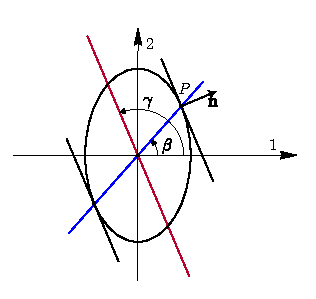
\includegraphics[scale=1.2]{figure/geometria_aree/coniugio_rette}
	\caption{Coniugio tra rette.}
	\label{fig:coniugiorette}
\end{figure}


Concludiamo allora che  vale la seguente \textit{relazione di coniugio}:
\begin{definition}\label{tanbg}
	\begin{equation}
\tan \beta \tan \gamma=-\frac{\rho_1^2}{\rho_2^2}.
\end{equation}
\end{definition}


\begin{remark}
Non esistono rette auto-coniugate. Infatti se la retta di pendenza $\alpha$ fosse auto-coniugata varrebbe
\begin{equation}
(\tan\alpha)=-\frac{\rho_1^2}{\rho_2^2},
\end{equation}
che è evidentemente impossibile.
\end{remark}

\subsection{Coniugio tra punti e rette: polarità e antipolarità}\label{polarità}
È possibile istituire due corrispondenze tra rette e punti, subordinate all'ellisse, dette  \textit{polarità} e \textit{antipolarità}.

Dato un punto $P=(x_1(P),x_2(P))$ l'\textit{antipolare} di $P$ è la retta
\begin{equation}\label{antipolare}
\frac{x_1(P)}{\rho_2^2}\,x_1+ \frac{x_2(P)}{\rho_1^2}\,x_2+1=0,
\end{equation}
mentre l'\textit{polare} è la retta
\begin{equation}
	\frac{x_1(P)}{\rho_2^2}\,x_1+ \frac{x_2(P)}{\rho_1^2}\,x_2-1=0,
\end{equation}

Le relazioni sono spesso dette di polo-polare o antipolo-antipolare.


%Tracciando una retta per $P$ e $G$, indicando con $P_0$ l'intersezione con l'ellisse, polare e antipolare sono due rette simmetriche rispetto all'origine, parallele alla tangente all'ellisse in $P_0$; la polare si trova dalla stessa parte rispetto al punto $P$, dalla parte opposta l'antipolare.

\begin{figure}[h]
	\centering
	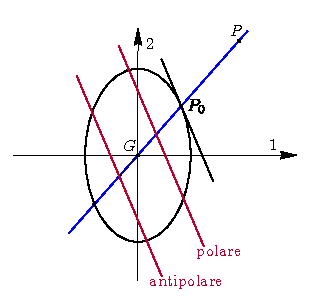
\includegraphics[scale=1.2]{figure/geometria_aree/polare}
	\caption{Coniugio di polarità e antipolarità.}
	\label{fig:polare}
\end{figure}

Vediamo alcune proprietà relative alla relazione di antipolarità.

\begin{enumerate}
	\item Non esistono coppie autoconiugate, ovvero non esistono antipolari contenenti il proprio antipolo, altrimenti si avrebbe
		\begin{equation}
			\frac{x^2_1(P)}{\rho_2^2}+ \frac{x^2_2(P)}{\rho_1^2}+1=0,
		\end{equation}
	che è impossibile.
\item L'antipolare è una retta parallela alla tangente nei punti di intersezione tra l'ellisse e la retta $x_2=\frac{x_2(P)}{x_1(P)}\,x_1$.
Infatti, abbiamo visto che a pendenza della retta tangente all'ellisse vale
\begin{equation}
	\bar{k}=-\frac 1k=-\frac{\rho_1^2}{\rho_2^2}\frac{x_1(P)}{x_2(P)}=\tan \gamma,
\end{equation}
che coincide con quella dell'antipolare  \eqref{antipolare}.
\item Se $P$ appartiene all'ellisse, allora l'antipolare è tangente all'ellisse in $-P=\big(-x_1(P),-x_2(P) \big)$, come è immediato verificare considerando la condizione di appartenenza all'ellisse e all'antipolare del punto $P_0$.
\item Se l'antipolo si avvicina all'origine, l'antipolare si allontana, se l'antipolo di allontana, l'antipolare si avvicina. Per vederlo conviene scrivere l'equazione dell'antipolare in forma segmentaria:
\begin{equation}
\frac{x_1}{p}+\frac{x_2}{q}=1,
\end{equation}
dove
\begin{equation}
(p, 0) \,\, {\rm e}\,\, (0,q)   \qquad p\coloneqq -\frac{\rho_2^2}{x_1(P)}, \qquad q\coloneqq -\frac{\rho_1^2}{x_2(P)}, 
\end{equation}
sono le intersezioni dell'antipolare con gli assi. Si vede allora che
\begin{itemize}
	\item Se $\big(x_1(P), x_2(P)\big)\to(0,0)$, allora $p\to-\infty$ e $q\to-\infty$, ovvero l'antipolare è una retta impropria;
	\item se l'antipolare passa per l'origine $p\to 0$ e $q\to 0$, allora $x_1(P)\to \infty$ e $x_2(P)\to \infty$, ovvero il centro è in punto all'infinito. 
\end{itemize}
Dunque l'antipolare di $G$ è la retta impropria e l'antipolo di una retta baricentrica è il punto improprio.
\end{enumerate}

Le proprietà 3 e 4 implicano che se $P$ è esterno all'ellisse, l'antipolare interseca l'ellisse; al contrario, se $P$ è interno, l'antipolare non interseca l'ellisse. Inoltre antipolo e antipolare si trovano da parti opposte rispetto all'origine.

	Per quanto riguarda invece la corrispondenza di polarità, osserviamo che esistono coppie autoconiugate. Con riferimento alla figura sotto,
\begin{center}
		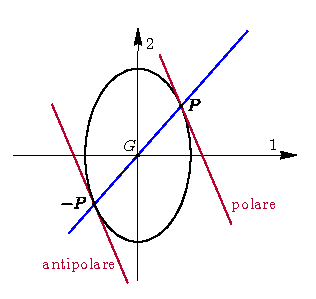
\includegraphics[scale=1.2]{figure/geometria_aree/antipolare}
\end{center}
il punto $P$ appartiene all'ellisse, dunque l'antipolare di $P$ è la retta tangente all'ellisse in $-P$; la polare allora passa per $P$ e dunque contiene il suo polo. Concludiamo che tutte le rette tangenti all'ellisse sono autoconiugate ai punti di tangenza nella corrispondenza di polarità.
Possiamo quindi concludere che l'ellisse d'inerzia è il luogo di poli autoconiugati nella polarità, ovvero l'inviluppo delle rette autoconiugate. 


Vale dunque il seguente corollario: sia $P$ l'antipolo di $r$.
\begin{center}
	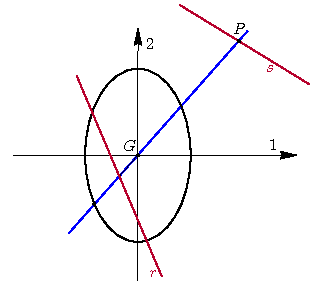
\includegraphics[scale=1.2]{figure/geometria_aree/corollario}
\end{center}
Allora le rette del fascio di sostegno $P$ sono le antipolari dei punti di $r$. 

Infine segnaliamo che vale il seguente \textit{teorema di reciprocità}:
Siano $(X, x)$ e $(Y, y)$ due coppie antipolo-antipolare (o polo-polare). Allora
\begin{equation}
	Y\in x \quad \Longleftrightarrow \quad X\in y.
\end{equation}
Infatti la retta $x$ antipolare di $X$ ha equazione
\begin{equation}
	\frac{x_1(X)}{\rho_2^2}\,x_1+ \frac{x_2(X)}{\rho_1^2}\,x_2+1=0;
\end{equation}
se $Y\in x$, allora
\begin{equation}\label{rec}
\frac{x_1(X)}{\rho_2^2}\,x_1(Y)+ \frac{x_2(X)}{\rho_1^2}\,x_2(Y)+1=0.
\end{equation}
D'altra parte, l'antipolare $y$ associata a $Y$ ha equazione 
\begin{equation}
	\frac{x_1(Y)}{\rho_2^2}\,x_1+ \frac{x_2(Y)}{\rho_1^2}\,x_2+1=0;
\end{equation}
poiché vale \eqref{rec}, concludiamo che $X\in y$.

\subsubsection{Costruzioni grafiche}
Proponiamo adesso delle costruzioni grafiche per determinare poli, antipoli, polari e antipolari.

\begin{enumerate}
	\item Determinare l'antipolare $p$ di un punto $P$ appartenente ad un asse coordinato.
	\begin{center}
		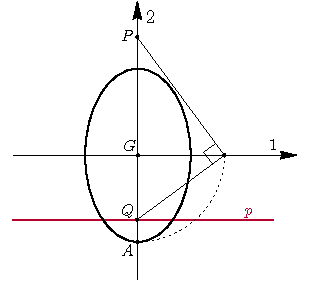
\includegraphics[scale=1.2]{figure/geometria_aree/costrgraf}
	\end{center}
Supponiamo che il punto $P$ abbia coordinata $\big(0, x_2(P) \big)$. L'equazione dell'antipolare è allora
\begin{equation}
\frac{x_2(P) }{\rho_1^2}x_2+1=0 \qquad \Longleftrightarrow \qquad -\frac{x_2}{\rho_1}=\frac{\rho_1}{x_2(P)}.
\end{equation}
Dunque $\rho_1=|\overrightarrow{GA}|$ è medio proporzionale tra $|\overrightarrow{GQ}|$ e $|\overrightarrow{GP}|$. Possiamo allora usare il secondo teorema di Euclide\footnote{In un triangolo rettangolo, l'altezza relativa all'ipotenusa è media proporzionale tra i segmenti in cui l'ipotenusa è divisa dalla stessa altezza.} e costruire il triangolo rettangolo rappresentato il figura, che fornisce la posizione del punto $Q$ da cui passa l'antipolare. Essendo $P$ sull'asse $x_1=0$, l'antipolare sarà parallela all'asse $x_1$.
\item Determinare l'antipolare di un  punto esterno all'ellisse. 
	\begin{center}
	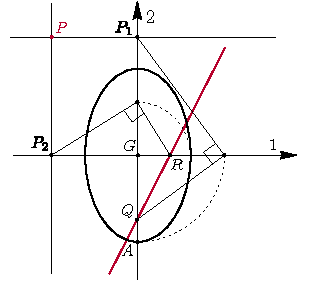
\includegraphics[scale=1.2]{figure/geometria_aree/costrgraf1}
\end{center}
Sfruttando la costruzione precedente, possiamo determinare gli antipoli $Q$ e $R$ delle rette passanti per $P$ e parallele agli assi coordinati. Per il teorema di reciprocità l'antipolare di $P$ è la retta passante per $Q$ e $R$.
\item Determinare la polare di un punto $P$ esterno all'ellisse.
	\begin{center}
	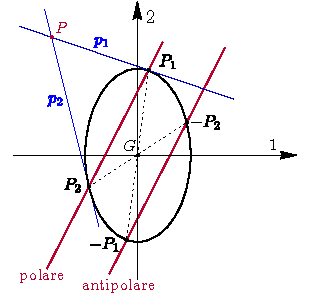
\includegraphics[scale=1.2]{figure/geometria_aree/costrgraf2}
\end{center}
Si traccino da $P$ le rette tangenti all'ellisse $p_1$ e $p_2$. Il punto $P_1$ è il polo di $p_1$ e il punto $P_2$ il polo di $P_2$. Per il teorema di reciprocità, dato che $P\in p_1$, $P_1$ si trova sulla polare di $P$; analogamente, dato che $P\in p_2$, $P_2$ si trova sulla polare di $P$. Pertanto la polare di $P$ è la retta passante per $P_1$ e $P_2$. L'antipolare invece passa per $-P_1$ e $-P_2$ 

\item Determinare l'antipolare di un  punto interno all'ellisse. 
	\begin{center}
	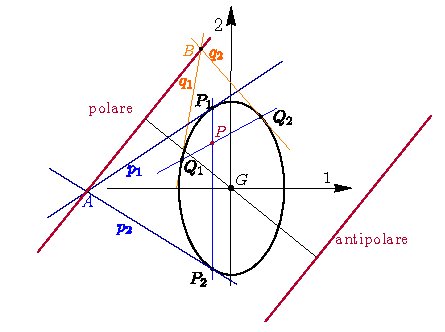
\includegraphics[scale=1.2]{figure/geometria_aree/costrgraf3}
\end{center}
In questo caso occorre tracciare due rette non parallele passanti per $P$. Partiamo dalla prima, che interseca l'ellisse nei punti $P_1$ e $P_2$. La retta $p_1$ tangente all'ellisse in $P_1$ è la polare di $P_1$ e la retta $p_2$ tangente all'ellisse in $P_2$ è la polare di $P_2$. Il punto di intersezione $A$ è allora il polo della retta passante per $P_1$ e $P_2$, per il teorema di reciprocità. Analogamente il punto $B$ è il polo della retta passante per $Q_1$ e $Q_2$. Se segue che la retta per $A$ e $B$ è la polare di $P$. L'antipolare si trova invece dalla parte opposta al baricentro, alla stessa distanza.
\end{enumerate}
%
%\newpage
%
%\begin{table}[h!]
%	\centering
%	\begin{tabular}{|c|c|c|c|}
%		\hline
%		\textbf{Forma} & \textbf{Area (A)} & \textbf{Baricentro (G)} & \textbf{Momenti d'inerzia e centrifughi (I)} \\ 
%		\hline
%		
%		\multirow{2}{*}{\begin{tikzpicture}[scale=0.5]
%				\draw (0,0) rectangle (2,1);
%		\end{tikzpicture}} & \multirow{2}{*}{$b \cdot h$} & $x(G) = \frac{b}{2}$ & $I_x = \frac{b h^3}{12}$ \\
%		& & $y(G) = \frac{h}{2}$ & $I_y = \frac{h b^3}{12}, \, I_{xy} = 0$ \\
%		\hline
%		
%		\multirow{2}{*}{\begin{tikzpicture}[scale=0.5]
%				\draw (0,0) -- (2,0) -- (1,1.5) -- cycle;
%		\end{tikzpicture}} & \multirow{2}{*}{$\frac{b \cdot h}{2}$} & $x(G) = \frac{b}{3}$ & $I_x = \frac{b h^3}{36}$ \\
%		& & $y(G) = \frac{h}{3}$ & $I_y = \frac{h b^3}{36}, \, I_{xy} = -\frac{b^2 h^2}{72}$ \\
%		\hline
%		
%		\multirow{2}{*}{\begin{tikzpicture}[scale=0.5]
%				\draw (0,0) -- (2,0) -- (2,1.5) -- cycle;
%		\end{tikzpicture}} & \multirow{2}{*}{$\frac{b \cdot h}{2}$} & $x(G) = \frac{b}{3}$ & $I_x = \frac{b h^3}{36}$ \\
%		& & $y(G) = \frac{h}{3}$ & $I_y = \frac{h b^3}{36}, \, I_{xy} = 0$ \\
%		\hline
%		
%		\multirow{1}{*}{\begin{tikzpicture}[scale=0.5]
%				\draw (0,0) circle (1);
%		\end{tikzpicture}} & $\pi r^2$ & $x(G) = 0$ & $I_x = I_y = \frac{\pi r^4}{4}, \, I_{xy} = 0$ \\
%		& & $y(G) = 0$ &  \\
%		\hline
%		
%		\multirow{2}{*}{\begin{tikzpicture}[scale=0.5]
%				\draw (0,0) arc (0:180:1cm) -- (-2,0) -- cycle;
%		\end{tikzpicture}} & \multirow{2}{*}{$\frac{\pi r^2}{2}$} & $x(G) = 0$ & $I_x = \frac{\pi r^4}{8}$ \\
%		& & $y(G) = \frac{4r}{3\pi}$ & $I_y = \frac{\pi r^4}{8}, \, I_{xy} = 0$ \\
%		\hline
%		
%		\multirow{2}{*}{\begin{tikzpicture}[scale=0.5]
%				\draw (0,0) ellipse (2cm and 1cm);
%		\end{tikzpicture}} & \multirow{2}{*}{$\pi a b$} & $x(G) = 0$ & $I_x = \frac{\pi ab^3}{4}$ \\
%		& & $y(G) = 0$ & $I_y = \frac{\pi a^3b}{4}, \, I_{xy} = 0$ \\
%		\hline
%		
%	\end{tabular}
%	\caption{Proprietà geometriche delle forme più comuni, con disegni, baricentro e momenti d'inerzia.}
%	\label{tab:geometric_properties}
%\end{table}